\chapter{Implémentation}
\label{chap:implementation}

Ce chapitre décrit les choix techniques et les décisions d'implémentation du pipeline.
Les résultats expérimentaux sont présentés au chapitre~\ref{chap:resultats}.

% ─────────────────────────────────────────────────────────────────────────────
\section{Environnement technique}
% ─────────────────────────────────────────────────────────────────────────────

\subsection{Infrastructure de calcul}

Les expériences ont été conduites sur la plateforme Kaggle Notebooks, qui met à
disposition des ressources GPU sans nécessiter de configuration locale. Ce choix
s'impose par deux contraintes pratiques~: l'accès gratuit à deux GPU NVIDIA Tesla T4
et la disponibilité directe du dataset BRFSS via l'API \texttt{kagglehub}, évitant
un téléchargement manuel de 350~Mo. Le tableau~\ref{tab:env} liste les spécifications
de l'environnement utilisé.

\begin{table}[H]
\centering
\caption{Spécifications de l'environnement d'exécution (Kaggle Notebooks, mai 2026)}
\label{tab:env}
\begin{tabular}{ll}
\toprule
\textbf{Composant} & \textbf{Spécification} \\
\midrule
Plateforme  & Kaggle Notebooks \\
GPU         & NVIDIA Tesla T4 $\times$ 2 (13\,757 Mo VRAM chacun) \\
RAM         & 29 Go (mode GPU activé) \\
Stockage    & 20 Go (espace de travail \texttt{/kaggle/working/}) \\
CPU         & 4 cœurs Intel Xeon \\
\bottomrule
\end{tabular}
\end{table}

\subsection{Stack technologique}

\begin{table}[H]
\centering
\caption{Stack logicielle du projet}
\label{tab:stack}
\begin{tabular}{ll}
\toprule
\textbf{Composant}       & \textbf{Technologie / Version} \\
\midrule
Langage                  & Python 3.10 (Kaggle) \\
Traitement distribué     & Apache Spark 4.0.2 (PySpark) \\
Deep Learning            & TensorFlow 2.19.0 / Keras 3 \\
Machine Learning         & XGBoost 3.2.0, scikit-learn 1.3 \\
Visualisation            & Matplotlib 3.7, Seaborn 0.12, Plotly 5.15 \\
Dashboard                & Streamlit 1.28 \\
Format de données        & Parquet (Spark), CSV (pandas) \\
Stockage des modèles     & \texttt{.keras} (DNN), \texttt{.json} (XGBoost), \texttt{.pkl} (scaler) \\
\bottomrule
\end{tabular}
\end{table}

Spark 4.0.2 est utilisé en mode local (\texttt{local[*]})~: il exploite l'ensemble
des cœurs CPU disponibles via un exécuteur unique, sans cluster HDFS.
Ce mode est adapté aux volumes inférieurs à quelques dizaines de millions de lignes
sur une machine de 29~Go de RAM.

\subsection{Organisation du projet}

Le projet est structuré en six notebooks Kaggle numérotés, correspondant chacun
à une phase du pipeline~: chargement et nettoyage, analyse exploratoire,
feature engineering, entraînement DNN, entraînement XGBoost et Spark GBT, évaluation
comparative. Cette organisation modulaire garantit que chaque notebook peut être
exécuté indépendamment en chargeant les artefacts produits par les notebooks précédents.

Le tableau de bord Streamlit (\texttt{streamlit\_dashboard/}) est découplé des notebooks~:
il charge des artefacts pré-calculés (JSON, CSV, PNG) et peut être exécuté localement
sans infrastructure Spark ni modèle chargé en mémoire, depuis n'importe quelle version
de Python comprise entre 3.8 et 3.14.

% ─────────────────────────────────────────────────────────────────────────────
\section{Phase 1 : Ingestion et nettoyage des données}
% ─────────────────────────────────────────────────────────────────────────────

\subsection{Configuration de la session Spark}

La session Spark est initialisée en mode local (\texttt{local[*]}), allouant 8~Go
de mémoire au pilote et réduisant le nombre de partitions de shuffle de 200
(valeur par défaut) à~8, valeur adaptée à un environnement à 4~cœurs. Ce réglage
évite la prolifération de petites partitions inutiles lors des opérations de tri et
d'agrégation, réduisant l'overhead du scheduler Spark.

Le fichier \texttt{brfss\_2020\_2024\_pooled\_ml.parquet} (79,5~Mo) est chargé
directement en mémoire Spark avec mise en cache (\texttt{cache()}), permettant les
opérations suivantes de comptage et de filtrage sans relecture du disque.

\subsection{Pipeline de binarisation}

Comme décrit au chapitre~\ref{chap:methodologie} (section~3.3.1), le format BRFSS
utilise la convention $1 = \text{Oui}$, $2 = \text{Non}$ pour les variables
dichotomiques. La transformation est appliquée via l'API DataFrame de PySpark,
colonne par colonne, garantissant que chaque variable respecte le schéma binaire
$\{0{,}0~;~1{,}0\}$ attendu par les algorithmes de machine learning.

La variable cible \texttt{HeartDiseaseorAttack} est dérivée de la variable composite
\texttt{\_MICHD} (voir section~3.1.2)~; le BMI est converti depuis son stockage
en centièmes dans \texttt{\_BMI5}~; les codes spéciaux de MentHlth (88 = aucun
mauvais jour) sont normalisés à 0.

\subsection{Déduplication et contrôle qualité}

La déduplication est effectuée sur l'ensemble des 14 colonnes sélectionnées après
binarisation. Le dataset passe de 2\,176\,776 à 1\,760\,241 lignes, soit la
suppression de 416\,535 enregistrements dupliqués (19,1\% du total). Les doublons
proviennent du regroupement de cinq années d'enquête~: un même répondant déclarant
les mêmes valeurs sur deux années différentes génère deux lignes identiques.

Un contrôle qualité post-déduplication vérifie~: (1) l'absence de valeurs hors
de l'intervalle $\{0{,}0~;~1{,}0\}$ pour les variables binaires~; (2) la distribution
de la variable cible ($10{,}32\%$ de positifs)~; (3) l'absence de lignes entièrement
nulles.

\begin{figure}[H]
    \centering
    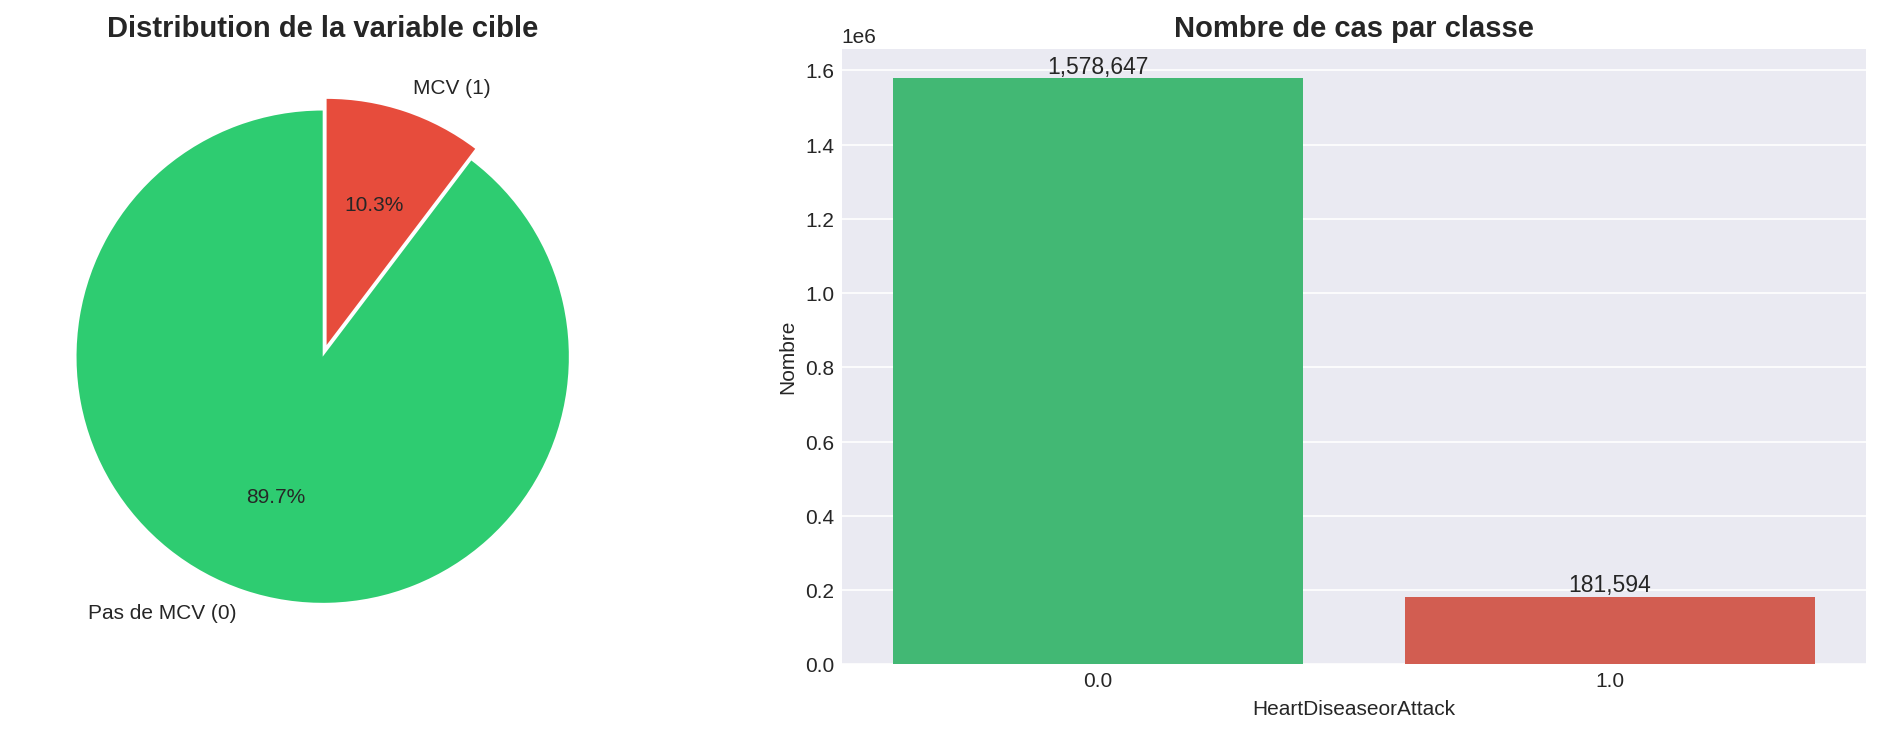
\includegraphics[width=0.80\textwidth]{figures/target_distribution.png}
    \caption{Distribution de la variable cible \texttt{HeartDiseaseorAttack}
             après nettoyage (1\,760\,241 observations). Le déséquilibre de classes
             (rapport 8,68~:~1) justifie la stratégie de pondération adoptée.}
    \label{fig:target_dist_impl}
\end{figure}

\begin{figure}[H]
    \centering
    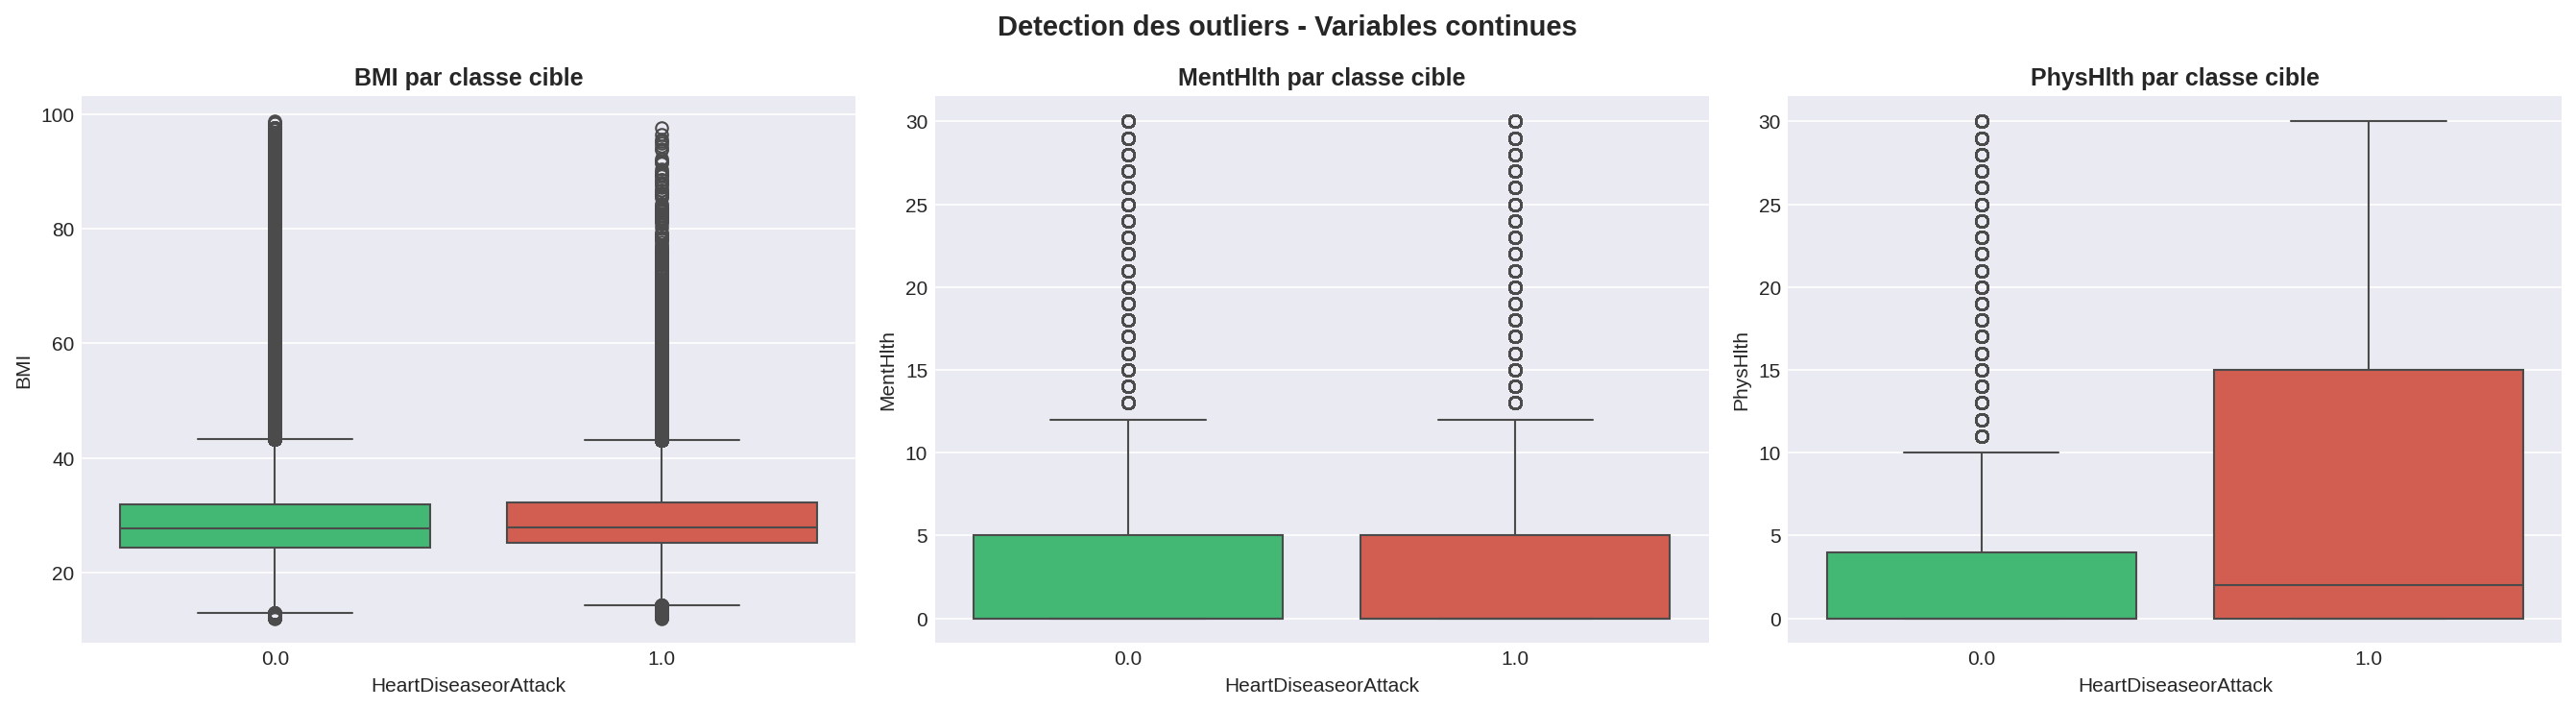
\includegraphics[width=\textwidth]{figures/outliers_boxplots.png}
    \caption{Distributions de BMI, MentHlth et PhysHlth selon la classe cible.
             Les valeurs de BMI atteignent 98,77~kg/m$^2$ (obésité morbide documentée~;
             conservées sans écrêtage). PhysHlth présente une séparation nette
             entre les classes, confirmant sa pertinence prédictive.}
    \label{fig:outliers}
\end{figure}

Les valeurs extrêmes de BMI (jusqu'à 98,77~kg/m$^2$) sont conservées sans écrêtage~:
elles correspondent à des cas d'obésité morbide documentés dans les données BRFSS
et leur suppression biaiserait la distribution de l'échantillon.

% ─────────────────────────────────────────────────────────────────────────────
\section{Phase 2 : Analyse exploratoire et imputation}
% ─────────────────────────────────────────────────────────────────────────────

\subsection{Imputation des valeurs manquantes}

Le DataFrame Spark est converti en DataFrame pandas après la déduplication.
L'imputation suit deux règles~: médiane pour les variables continues (BMI, MentHlth,
PhysHlth), mode pour les variables binaires et ordinales.

La variable \texttt{HvyAlcoholConsump} présente 53,32\% de valeurs manquantes~:
ce module est optionnel dans le questionnaire BRFSS et n'a pas été collecté chaque
année du dataset 2020--2024. Son mode (0, absence de binge drinking) est utilisé
pour l'imputation. Après imputation, aucune valeur nulle ne subsiste dans le jeu
de données.

\subsection{Analyse de la prévalence par sous-groupe}

La figure~\ref{fig:mcv_age} illustre l'évolution du taux de MCV par tranche d'âge
sur le dataset nettoyé. La progression monotone croissante de la prévalence
(de 0,9\% pour les 18--24~ans à 24,7\% pour les 80~ans et plus) constitue un test
de cohérence épidémiologique des données~: toute inversion ou plateau anormal
indiquerait un problème d'encodage ou de binarisation.

\begin{figure}[H]
    \centering
    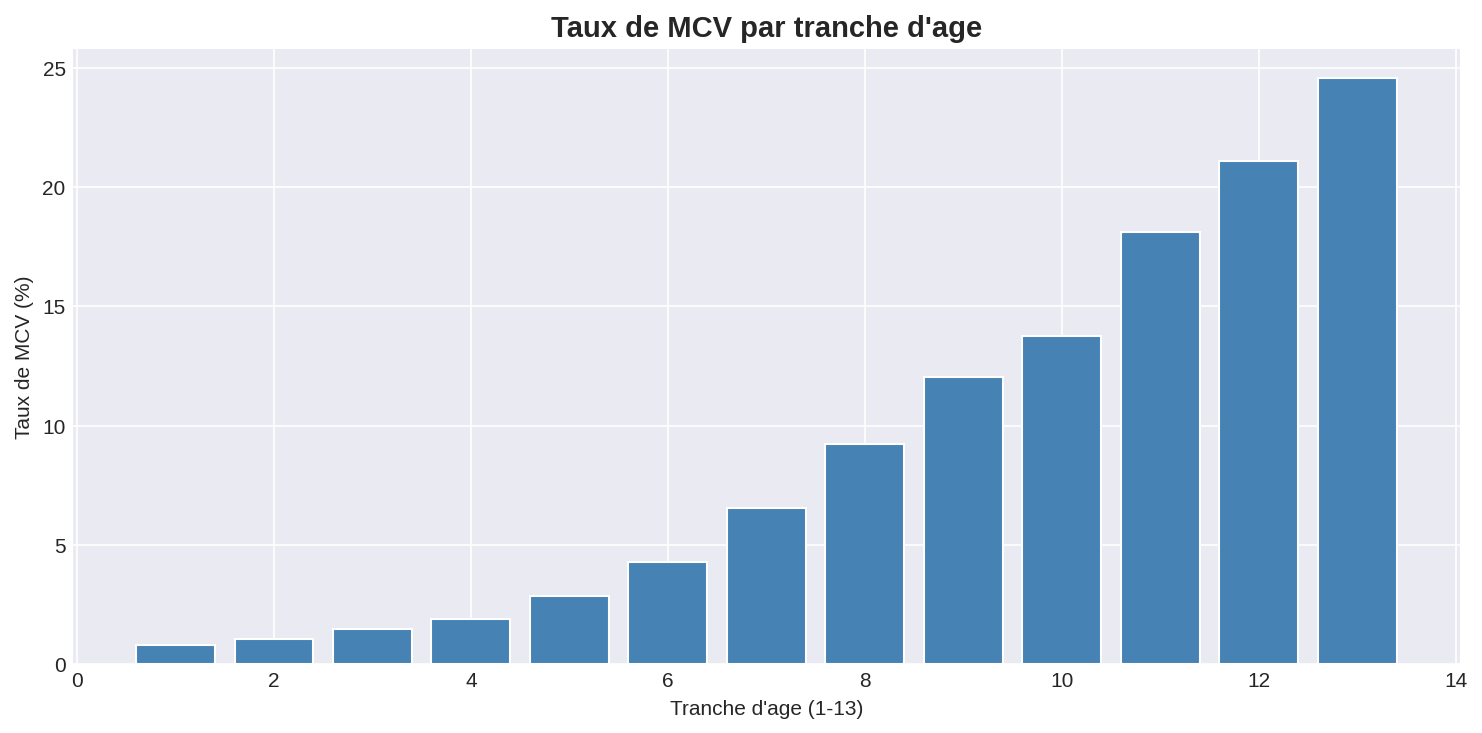
\includegraphics[width=0.85\textwidth]{figures/mcv_by_age.png}
    \caption{Taux de MCV par tranche d'âge (1 = 18--24 ans, 13 = 80 ans et plus).
             La progression est strictement croissante (0,9\% à 24,7\%),
             validant la cohérence épidémiologique du pipeline de binarisation.}
    \label{fig:mcv_age}
\end{figure}

% ─────────────────────────────────────────────────────────────────────────────
\section{Phase 3 : Feature Engineering et sélection des variables}
\label{sec:feature_engineering}
% ─────────────────────────────────────────────────────────────────────────────

\subsection{Analyse de corrélation avec la variable cible}

Les corrélations de Pearson et de Spearman sont calculées sur un échantillon
de 200\,000 lignes. Les matrices de corrélation complètes (figures~\ref{fig:corr_pearson}
et~\ref{fig:corr_spearman}) révèlent les structures d'association linéaires et
monotones entre l'ensemble des features.

\begin{figure}[H]
    \centering
    \begin{subfigure}[b]{0.48\textwidth}
        \centering
        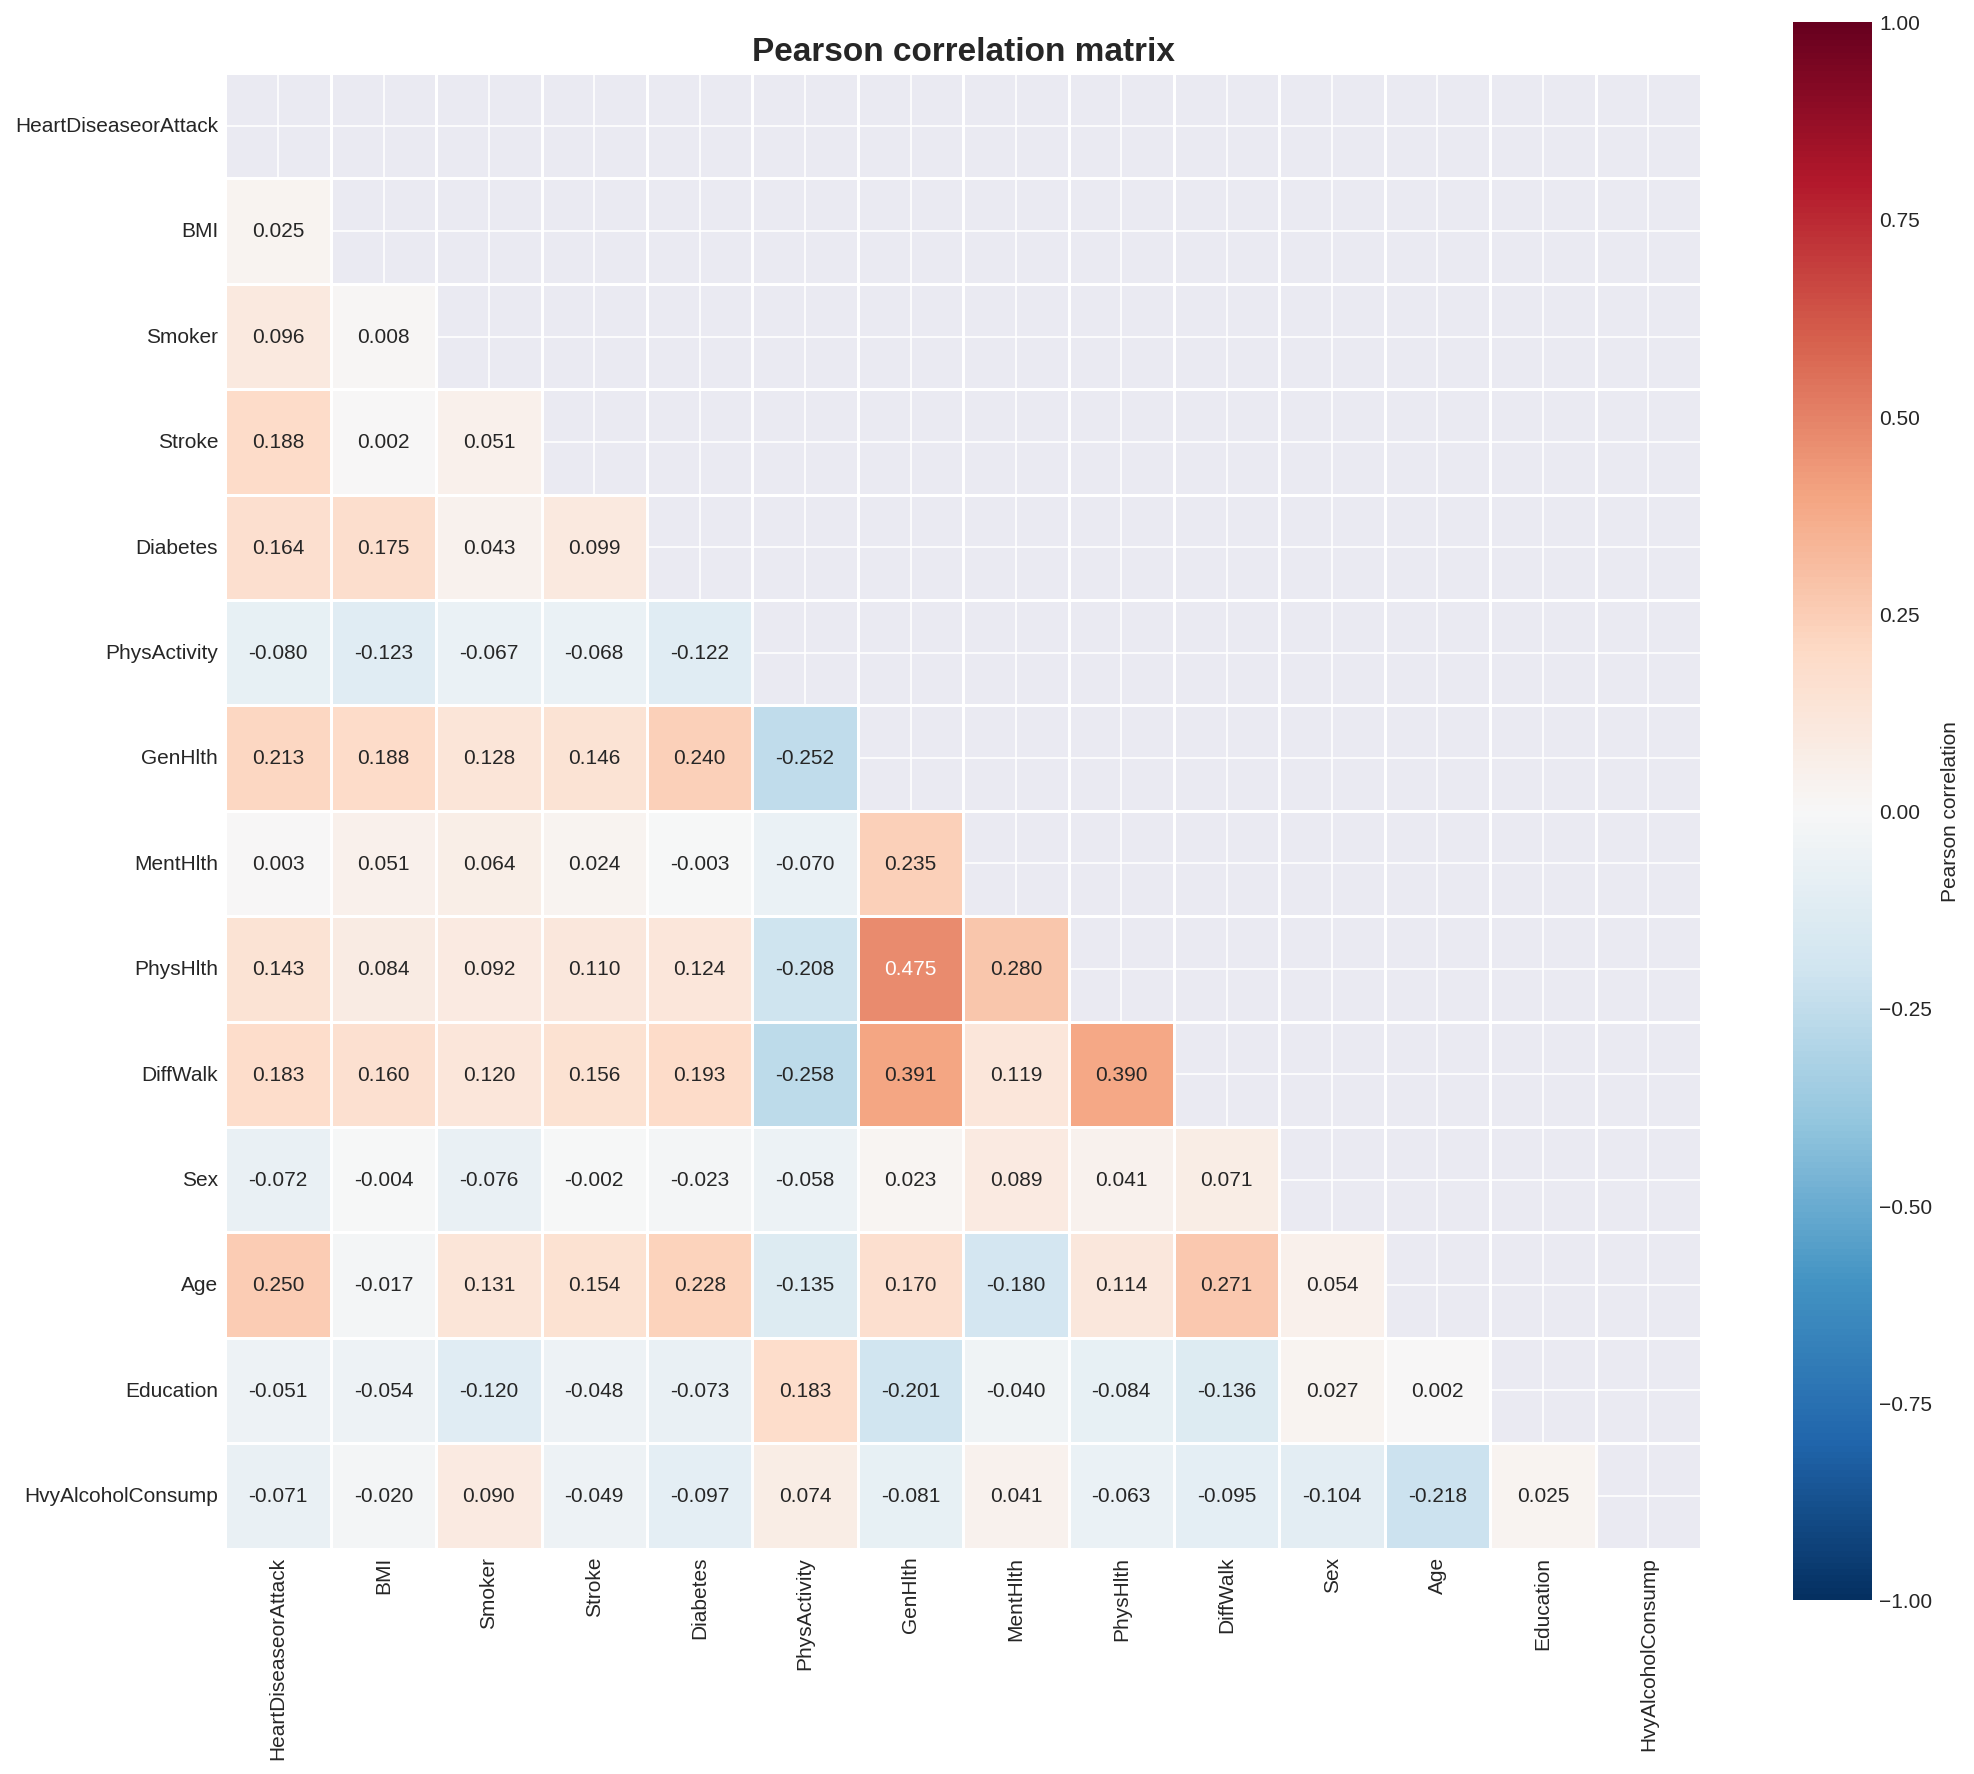
\includegraphics[width=\textwidth]{figures/corr_pearson.png}
        \caption{Corrélation de Pearson}
        \label{fig:corr_pearson}
    \end{subfigure}
    \hfill
    \begin{subfigure}[b]{0.48\textwidth}
        \centering
        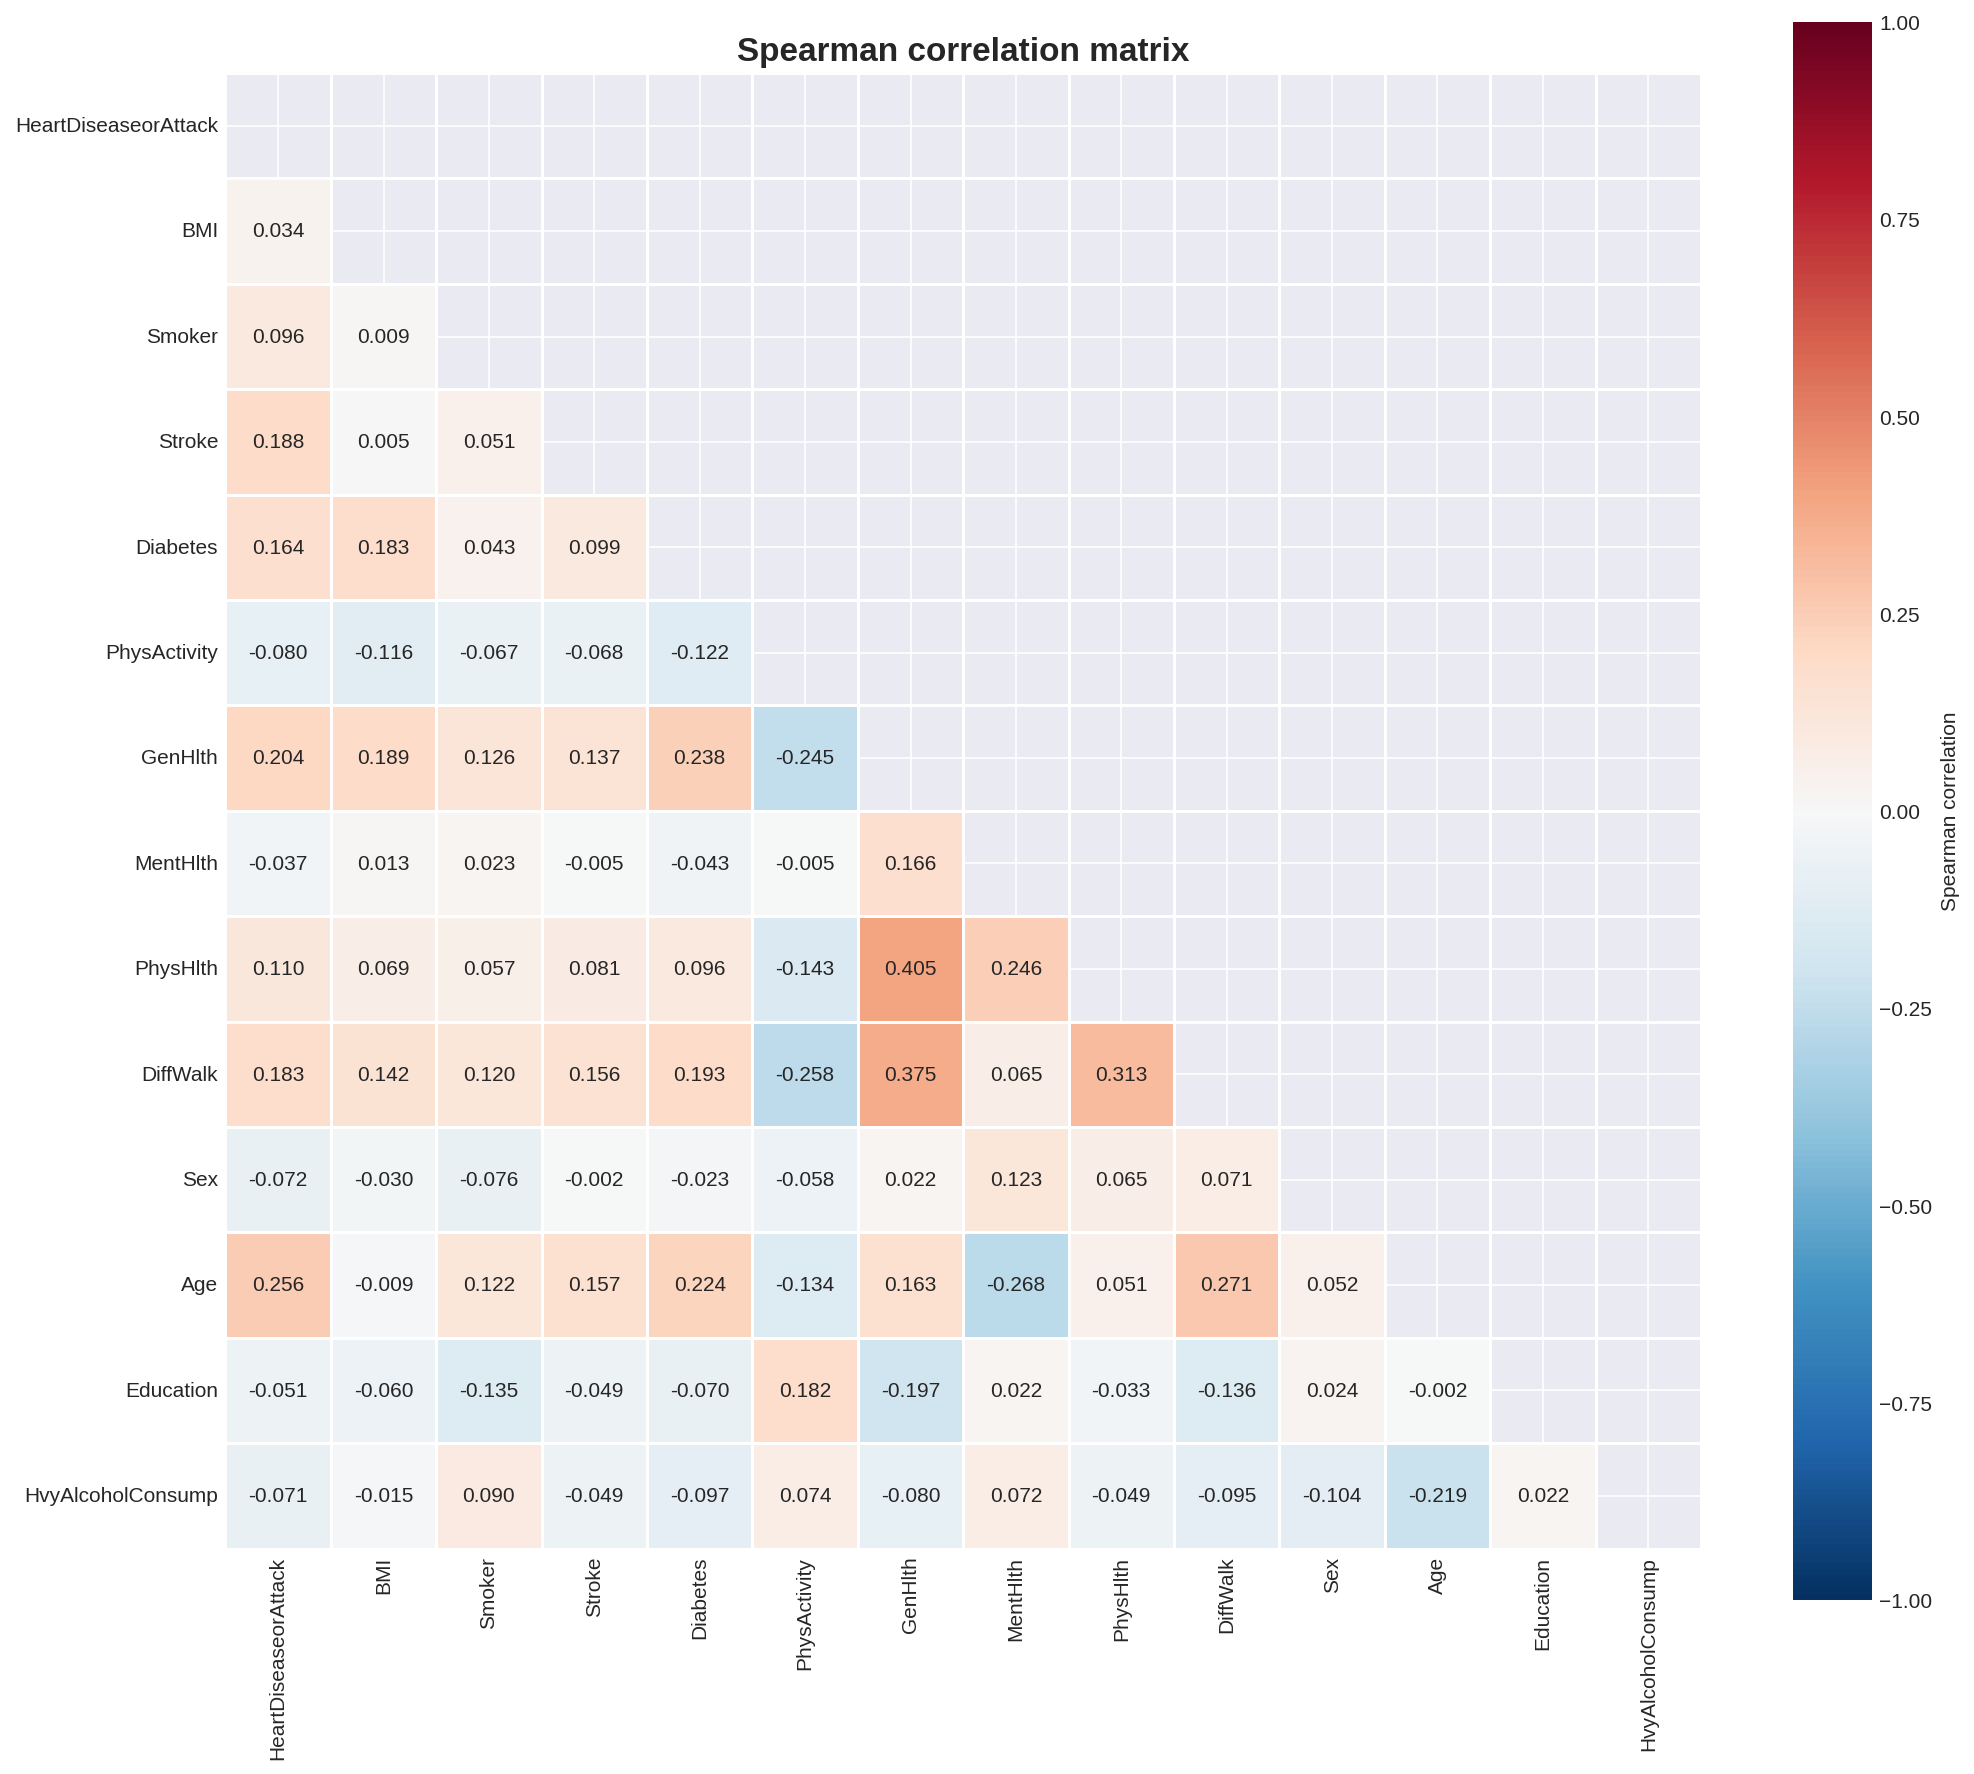
\includegraphics[width=\textwidth]{figures/corr_spearman.png}
        \caption{Corrélation de Spearman}
        \label{fig:corr_spearman}
    \end{subfigure}
    \caption{Matrices de corrélation de Pearson (linéaire) et de Spearman (monotone)
             sur les 15 features. Les deux méthodes convergent~: Age, GenHlth et Stroke
             présentent les corrélations les plus fortes avec la cible.}
    \label{fig:corr_matrices}
\end{figure}

La figure~\ref{fig:corr_comp} compare les deux mesures de corrélation avec la
variable cible feature par feature.

\begin{figure}[H]
    \centering
    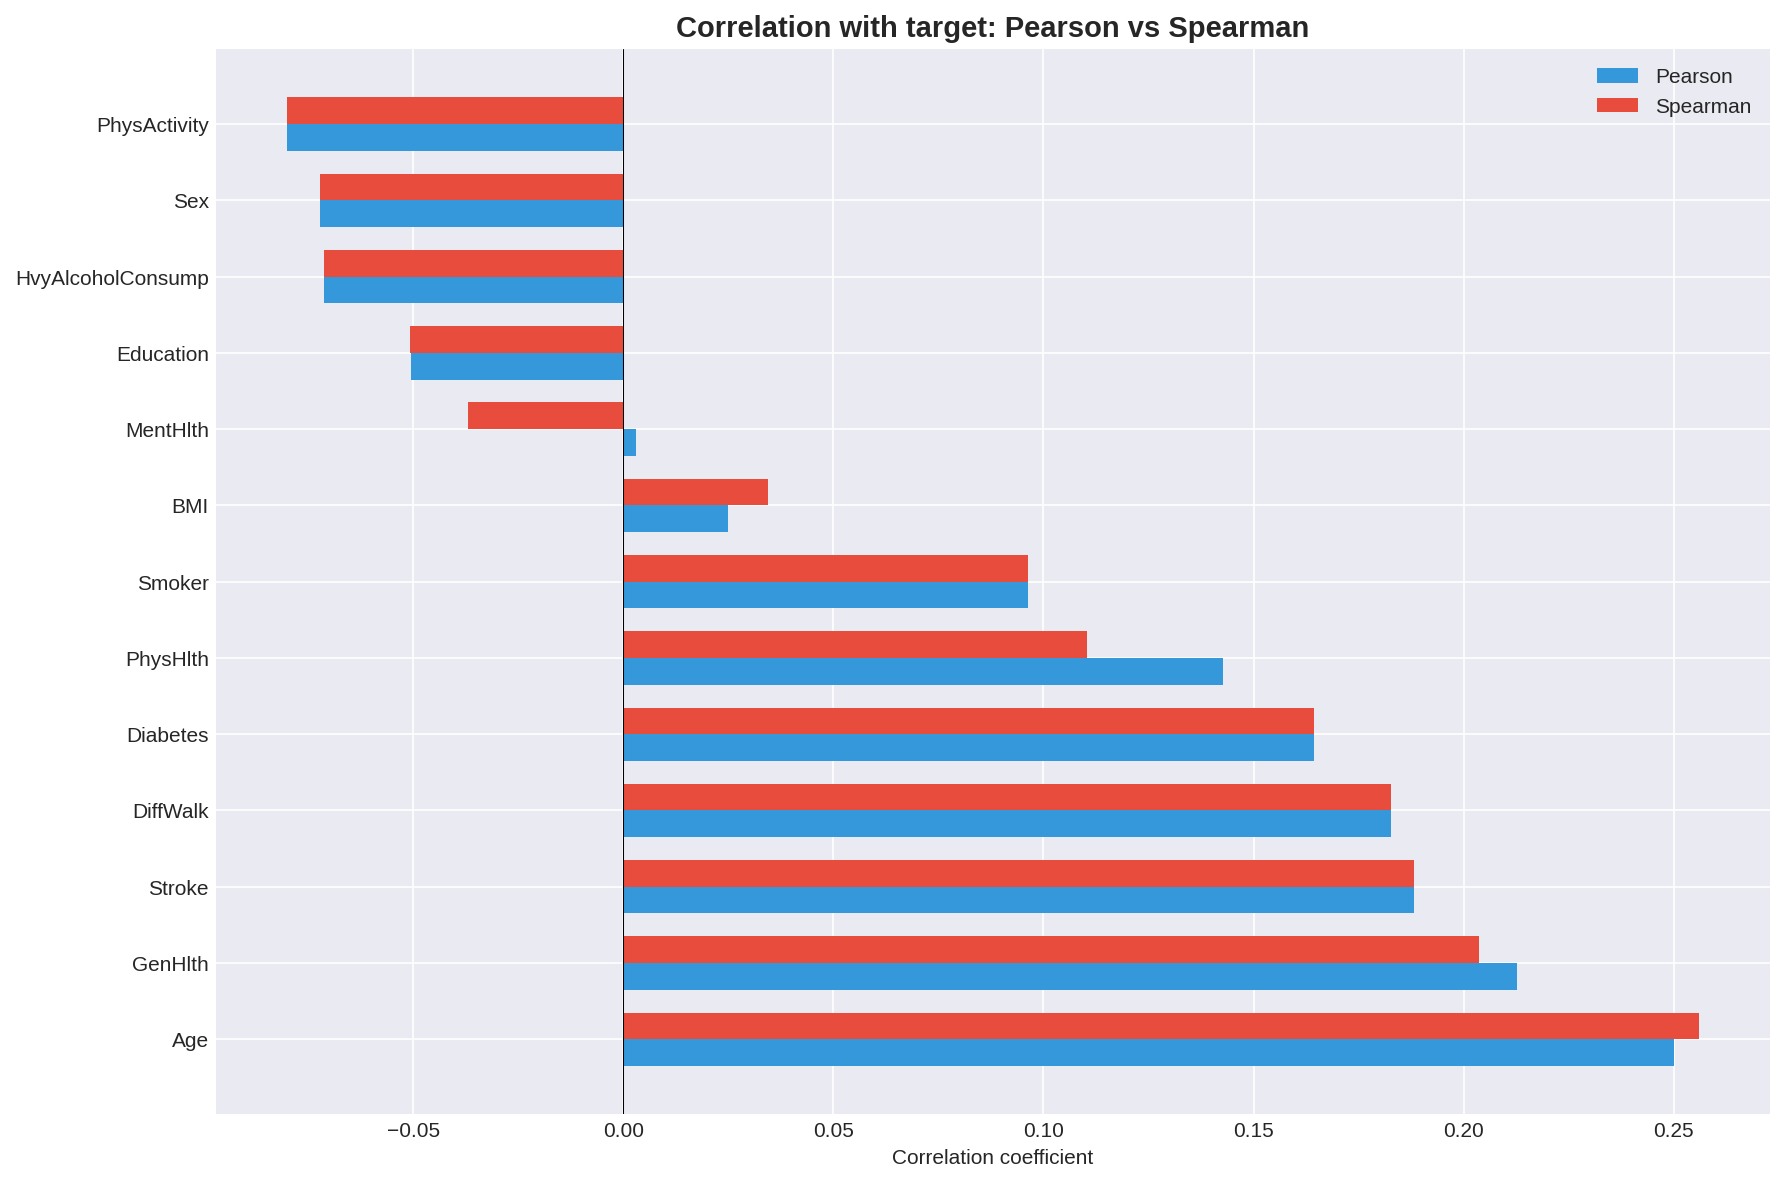
\includegraphics[width=0.90\textwidth]{figures/corr_comparison.png}
    \caption{Corrélations de Pearson et de Spearman avec la variable cible.
             Age, GenHlth et Stroke dominent les deux classements, confirmant
             leur pertinence clinique. MentHlth affiche une corrélation quasi nulle
             (+0,003 Pearson) malgré sa binarisation correcte~; HvyAlcoholConsump
             présente une corrélation négative ($-$0,07), attribuée au biais du
             survivant (\textit{survivor bias}).}
    \label{fig:corr_comp}
\end{figure}

\subsection{Importance Gini et test du $\chi^2$}

Un Random Forest de 100 arbres est entraîné sur 30\% de l'échantillon via Spark MLlib.
L'importance par réduction d'impureté de Gini et le V de Cramér (test du $\chi^2$)
sont calculés pour chaque feature. Le tableau~\ref{tab:feature_synthesis} synthétise
les rangs obtenus par les trois méthodes.

\begin{table}[H]
\centering
\caption{Synthèse multi-méthodes pour la sélection des features.
         Le rang moyen est calculé sur les méthodes disponibles pour chaque variable.}
\label{tab:feature_synthesis}
\begin{tabular}{lccccc}
\toprule
\textbf{Feature} & \textbf{Corr. Pearson} & \textbf{Rang corr.} &
\textbf{Gini} & \textbf{Rang Gini} & \textbf{Rang moyen} \\
\midrule
Age               & 0,250 & 1 & 0,341 & 1 & 1,0 \\
GenHlth           & 0,213 & 2 & 0,203 & 2 & 2,0 \\
Stroke            & 0,188 & 3 & 0,161 & 3 & 3,0 \\
DiffWalk          & 0,183 & 4 & 0,067 & 5 & 4,3 \\
Diabetes          & 0,164 & 5 & 0,068 & 4 & 4,7 \\
PhysHlth          & 0,143 & 6 & 0,033 & 7 & 6,5 \\
Smoker            & 0,096 & 7 & 0,019 & 8 & 7,0 \\
Sex               & 0,072 & 9 & 0,057 & 6 & 7,7 \\
PhysActivity      & 0,080 & 8 & 0,004 & 13 & 9,3 \\
HvyAlcoholConsump & 0,071 & 10 & 0,005 & 12 & 10,3 \\
BMI               & 0,025 & 12 & 0,019 & 9  & 10,5 \\
Education         & 0,051 & 11 & 0,010 & 11 & 10,7 \\
MentHlth          & 0,003 & 13 & 0,014 & 10 & 11,5 \\
\bottomrule
\end{tabular}
\end{table}

La convergence des trois méthodes sur le podium Age, GenHlth, Stroke renforce
la confiance dans la sélection finale. Toutes les associations sont statistiquement
significatives ($p < 10^{-100}$), la taille de l'échantillon (200\,000 lignes)
garantissant une puissance statistique maximale.

\begin{figure}[H]
    \centering
    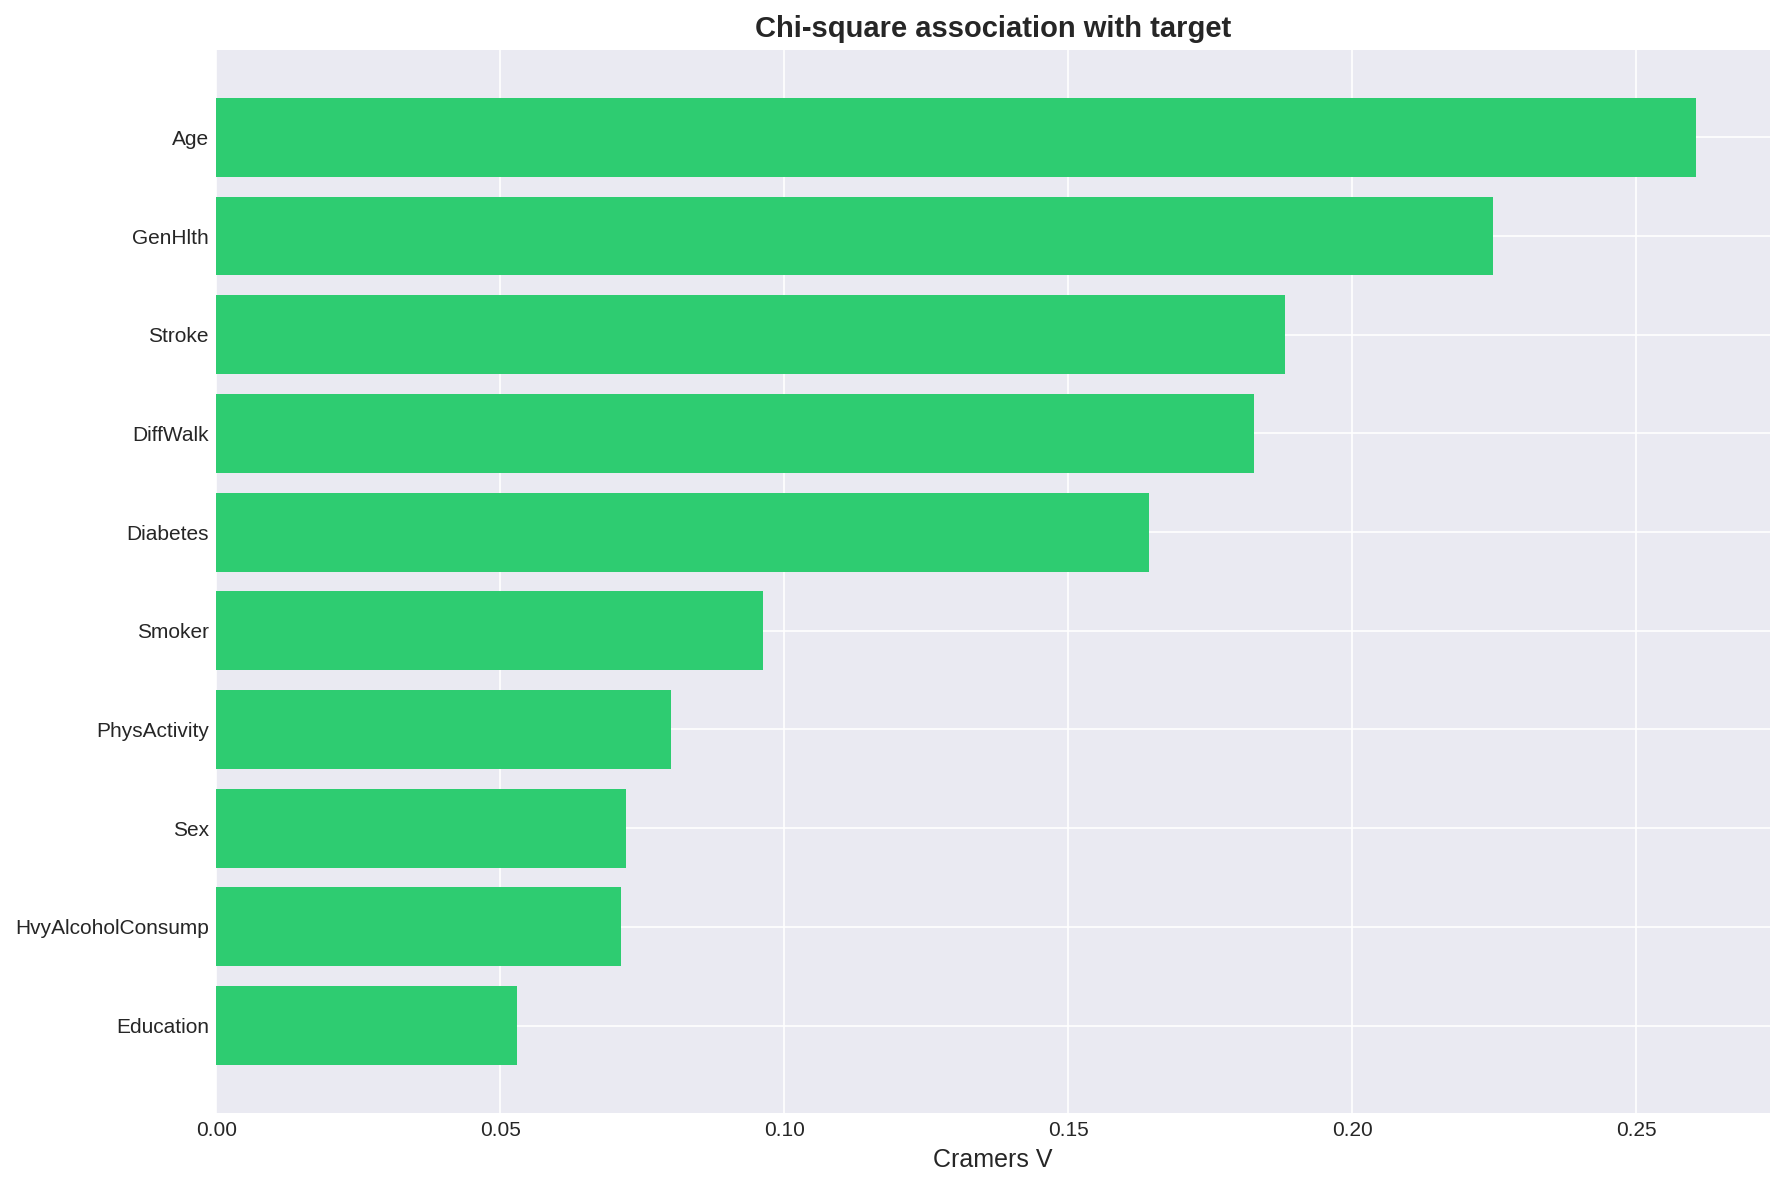
\includegraphics[width=0.80\textwidth]{figures/chi2_cramers_v.png}
    \caption{Association des variables catégorielles avec la variable cible
             (V de Cramér, test du $\chi^2$, $p \ll 0{,}05$ pour toutes les variables).
             Age et GenHlth obtiennent les V de Cramér les plus élevés (0,261 et 0,225),
             en concordance avec l'importance Gini.}
    \label{fig:chi2}
\end{figure}

\subsection{Variables dérivées}

Les deux features composites RiskScore et HealthIndex sont construites selon les
formules~(\ref{eq:riskscore}) et~(\ref{eq:healthindex}) du chapitre~\ref{chap:methodologie}.
Leur distribution selon la classe cible (figure~\ref{fig:derived}) montre une
séparation nette entre les groupes MCV et non-MCV, validant leur apport informatif.

\begin{figure}[H]
    \centering
    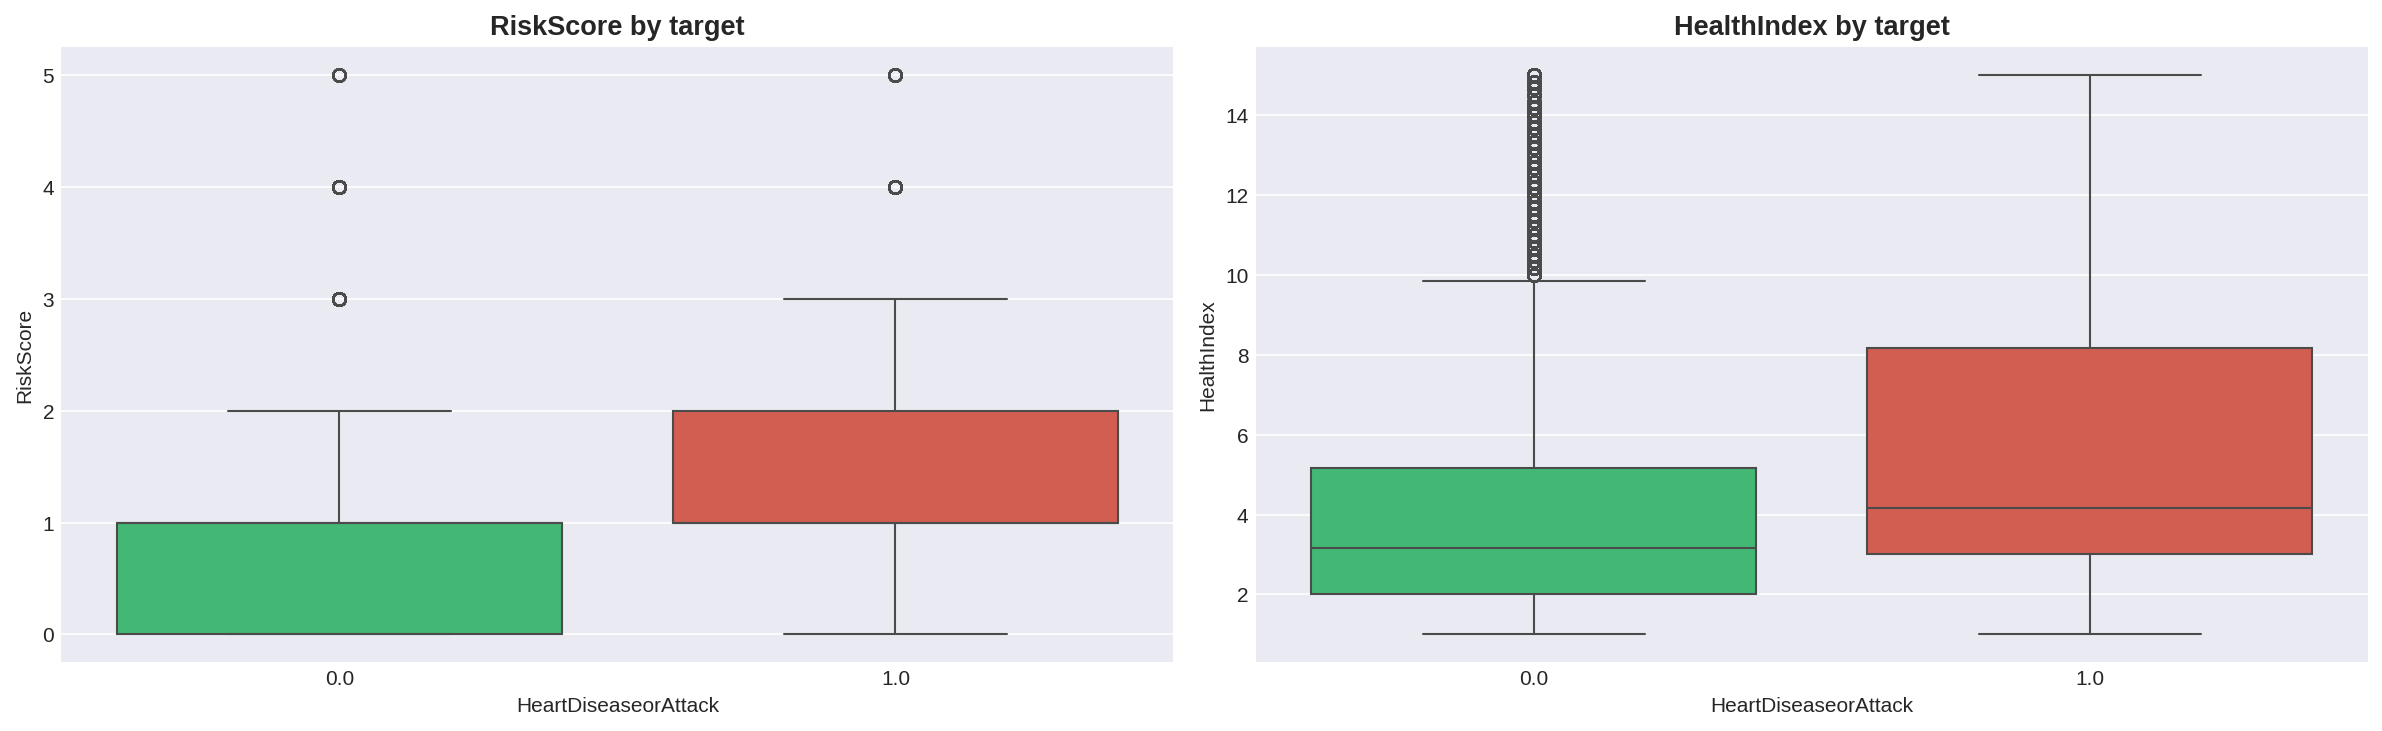
\includegraphics[width=0.90\textwidth]{figures/derived_features.png}
    \caption{Distributions de RiskScore (gauche) et HealthIndex (droite) selon
             la classe cible. Les deux variables présentent une séparation claire~:
             les patients MCV ont en moyenne un RiskScore plus élevé et un HealthIndex
             plus dégradé.}
    \label{fig:derived}
\end{figure}

\subsection{Analyse en composantes principales}

L'ACP est calculée sur les 13 features originales (sans RiskScore ni HealthIndex)
après application d'un filtre de variance (\texttt{VarianceThreshold($10^{-6}$)})
et d'une normalisation StandardScaler. La figure~\ref{fig:pca_analysis} présente
la variance expliquée cumulée par composante principale.

\begin{figure}[H]
    \centering
    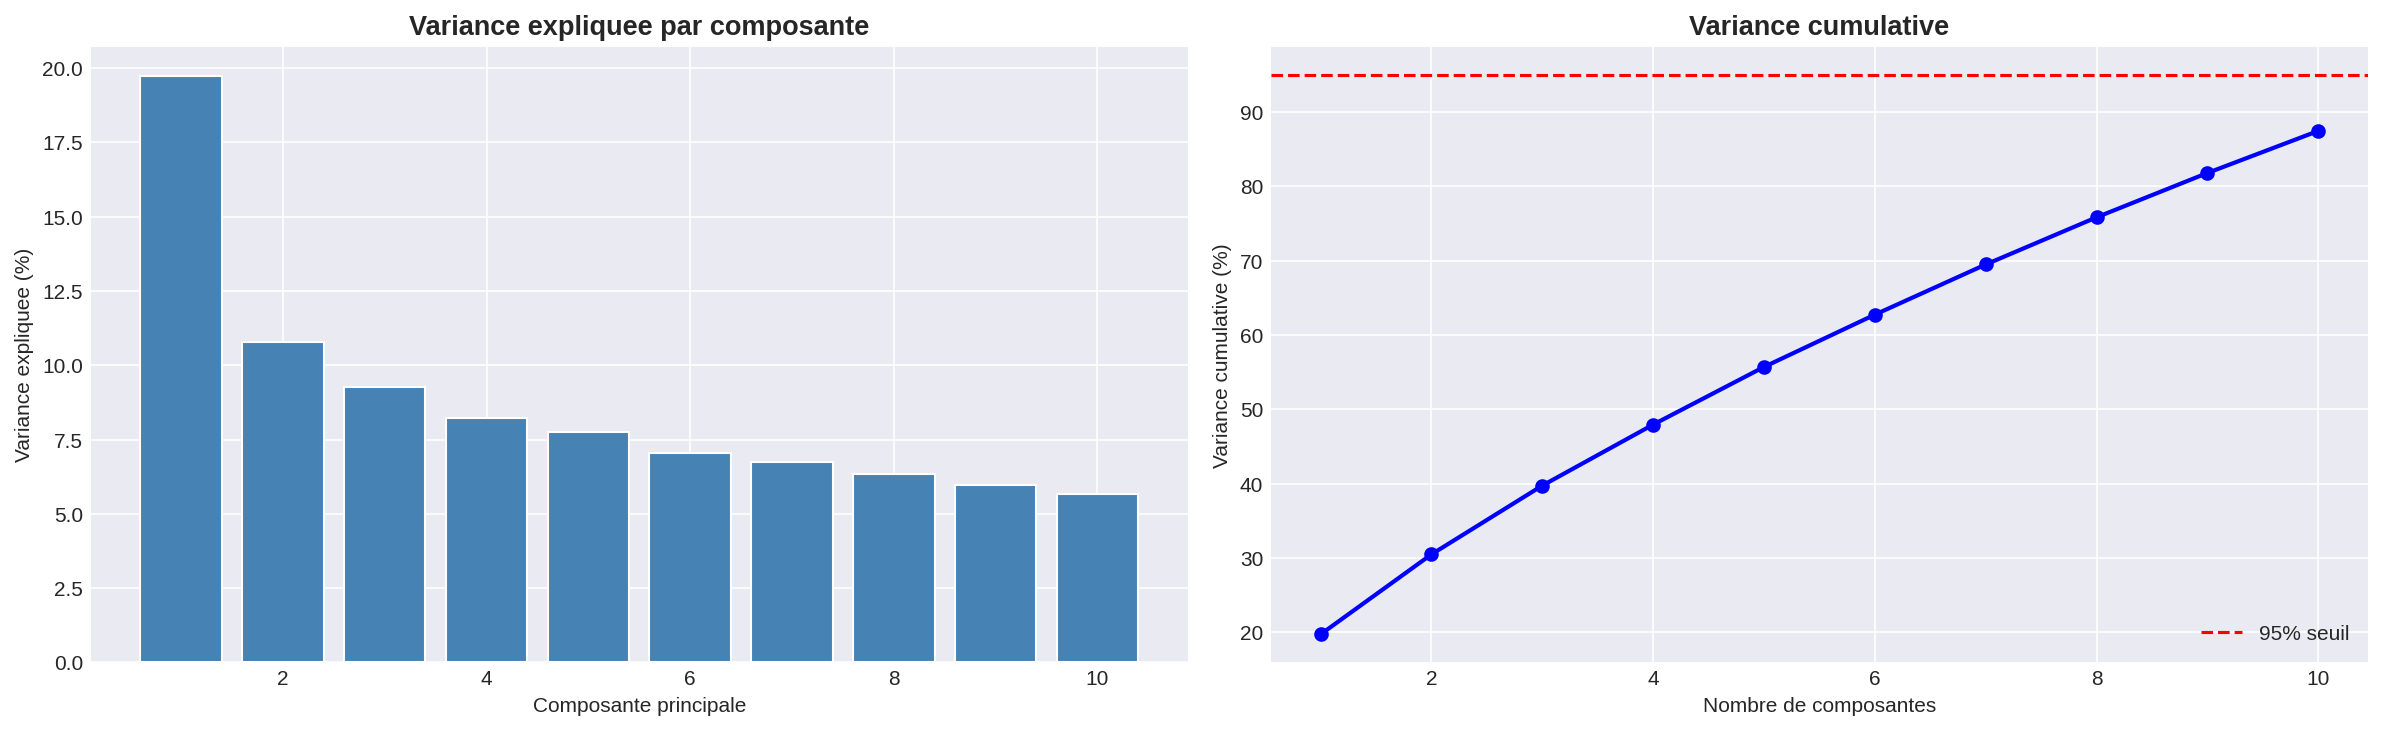
\includegraphics[width=\textwidth]{figures/pca_analysis.png}
    \caption{ACP sur les 13 features originales. Dix composantes expliquent 87,5\%
             de la variance totale. Le seuil de 95\% n'est pas atteint en 10
             composantes, ce qui reflète la nature hétérogène (binaire, ordinale,
             continue) des features BRFSS.}
    \label{fig:pca_analysis}
\end{figure}

La projection en 2D (figure~\ref{fig:pca_2d}) confirme l'absence de séparation
linéaire simple entre les classes, ce qui est cohérent avec un AUC-ROC de 0,82~:
aucune frontière de décision linéaire dans l'espace des deux premières composantes
ne peut atteindre de bonnes performances.

\begin{figure}[H]
    \centering
    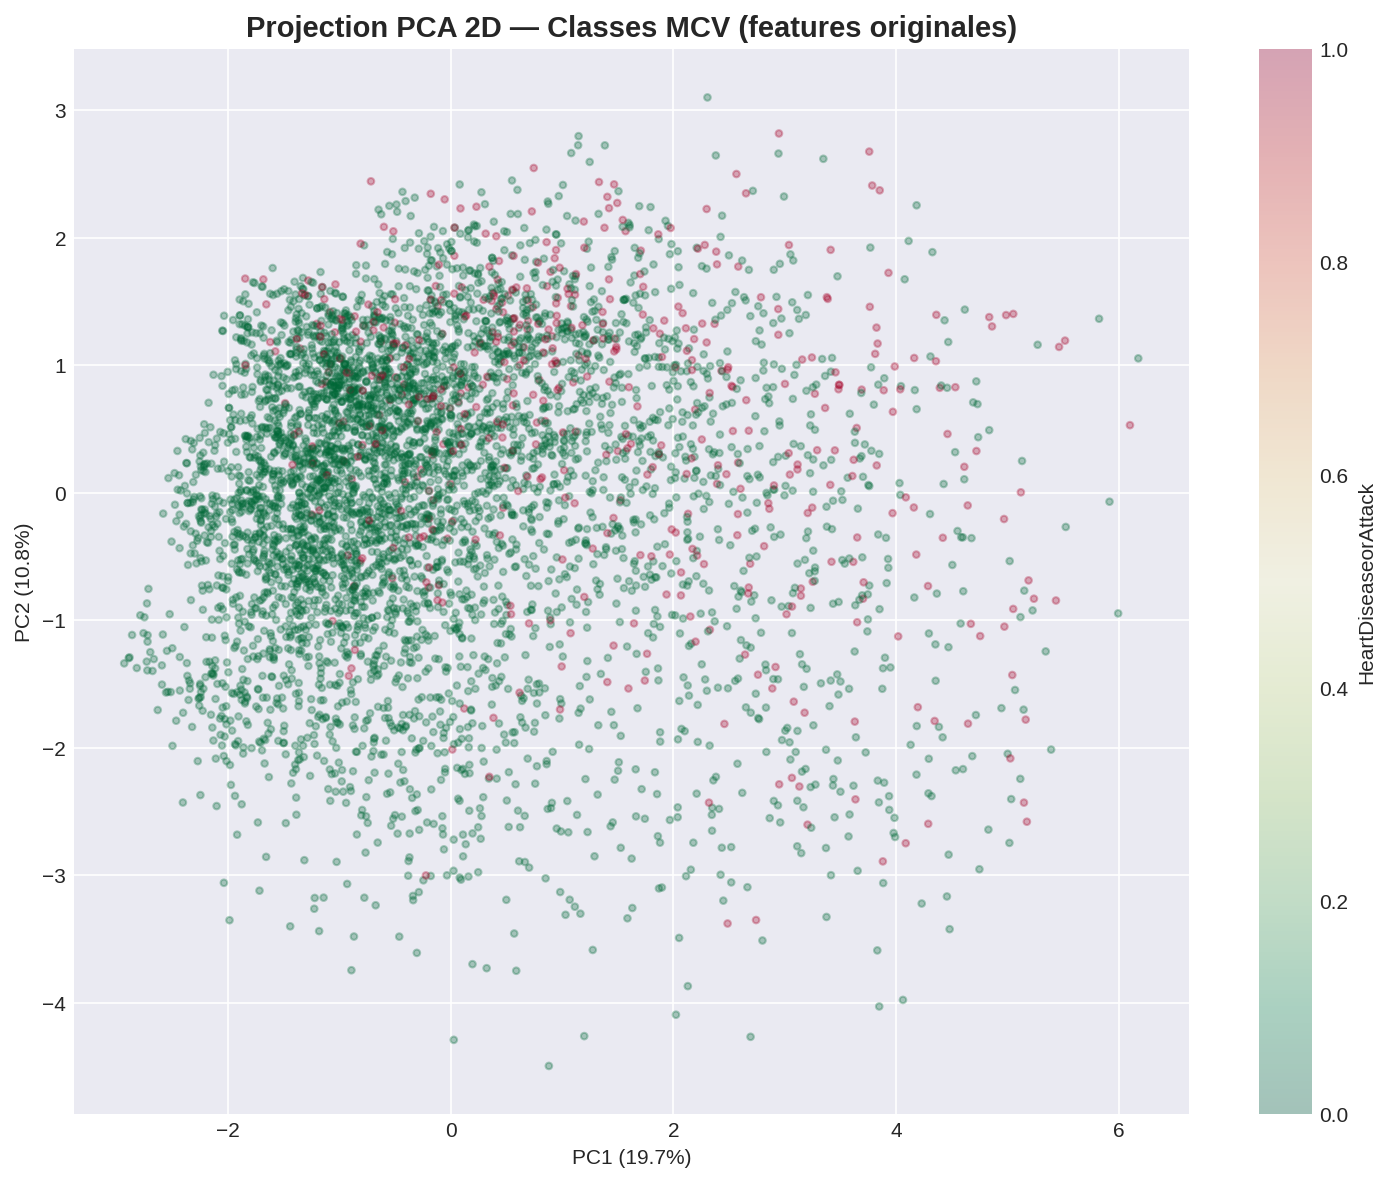
\includegraphics[width=0.60\textwidth]{figures/pca_2d.png}
    \caption{Projection 2D des 13 features originales (PC1 = 19,7\%, PC2 = 10,8\%).
             Les deux classes se superposent largement, justifiant le recours à des
             modèles non linéaires (DNN, XGBoost) plutôt qu'à une régression logistique.}
    \label{fig:pca_2d}
\end{figure}

L'ACP est utilisée exclusivement à titre exploratoire. Le pipeline de modélisation
conserve les 15 features sans réduction de dimension~: DNN et XGBoost traitent
efficacement cet espace, et la réduction de dimension introduirait une perte
d'interprétabilité clinique des features.

% ─────────────────────────────────────────────────────────────────────────────
\section{Phase 4 : Entraînement du réseau de neurones profond}
\label{sec:dnn}
% ─────────────────────────────────────────────────────────────────────────────

\subsection{Partitionnement stratifié et normalisation}

Le jeu de données est partitionné selon un schéma 70/15/15 (entraînement,
validation, test) avec stratification sur la variable cible, maintenant la
prévalence de 10,32\% dans chacune des trois partitions.

Le StandardScaler est ajusté exclusivement sur l'ensemble d'entraînement, puis
appliqué par transformation aux ensembles de validation et de test. Ce protocole
strict prévient toute fuite de données : les statistiques de normalisation
(moyenne, écart-type) ne doivent pas être informées par des exemples du jeu de test.

Les poids de classe sont calculés par la méthode \textit{balanced} sur les étiquettes
de l'ensemble d'entraînement uniquement~: $w_0 = 0{,}558$ (classe négative)
et $w_1 = 4{,}847$ (classe positive).

\subsection{Architecture et entraînement du DNN}

L'architecture du modèle est décrite dans le tableau~\ref{tab:dnn_arch_impl}.
Le réseau est implémenté en TensorFlow 2.19 / Keras~3, avec les composants
de régularisation suivants~:

\begin{table}[H]
\centering
\caption{Architecture du DNN (46\,849 paramètres entraînables)}
\label{tab:dnn_arch_impl}
\begin{tabular}{lrrl}
\toprule
\textbf{Couche} & \textbf{Unités} & \textbf{Paramètres} & \textbf{Remarques} \\
\midrule
Entrée (Dense)      & 256 & 4\,096  & ReLU, $L_2 = 10^{-4}$ \\
Batch Normalization & 256 & 1\,024  & normalisation des activations \\
Dropout             &  -- &     0   & taux = 0,30 \\
Dense               & 128 & 32\,896 & ReLU, $L_2 = 10^{-4}$ \\
Batch Normalization & 128 &   512   & normalisation des activations \\
Dropout             &  -- &     0   & taux = 0,30 \\
Dense               &  64 & 8\,256  & ReLU \\
Sortie (Dense)      &   1 &    65   & Sigmoïde \\
\midrule
\multicolumn{2}{l}{Total paramètres} & 46\,849 & (46\,081 entraînables) \\
\bottomrule
\end{tabular}
\end{table}

Le listing~\ref{lst:dnn_arch} présente la définition de l'architecture en
TensorFlow/Keras, seul extrait de code jugé nécessaire pour illustrer les
choix d'implémentation.

\begin{lstlisting}[caption={Architecture du DNN (TensorFlow 2.19 / Keras 3)},
                   label=lst:dnn_arch]
import tensorflow as tf
from tensorflow.keras import layers, regularizers

def build_dnn(input_dim):
    model = tf.keras.Sequential([
        tf.keras.Input(shape=(input_dim,)),
        layers.Dense(256, activation='relu',
                     kernel_regularizer=regularizers.l2(1e-4)),
        layers.BatchNormalization(),
        layers.Dropout(0.3),
        layers.Dense(128, activation='relu',
                     kernel_regularizer=regularizers.l2(1e-4)),
        layers.BatchNormalization(),
        layers.Dropout(0.3),
        layers.Dense(64, activation='relu'),
        layers.Dense(1, activation='sigmoid')
    ])
    model.compile(
        optimizer=tf.keras.optimizers.Adam(learning_rate=1e-3),
        loss='binary_crossentropy',
        metrics=['accuracy',
                 tf.keras.metrics.AUC(name='auc'),
                 tf.keras.metrics.Precision(name='precision'),
                 tf.keras.metrics.Recall(name='recall')]
    )
    return model
\end{lstlisting}

Deux callbacks contrôlent l'entraînement~: EarlyStopping (patience~=~5, suivi de
val\_auc, avec restauration des meilleurs poids) arrête l'entraînement lorsque
l'AUC de validation cesse de progresser~; ReduceLROnPlateau réduit le taux
d'apprentissage d'un facteur 0,5 lorsque la perte de validation stagne pendant
3 epochs consécutives, jusqu'à un minimum de $10^{-6}$.

L'entraînement s'est déroulé sur 36 epochs (taille de lot 1\,024), le meilleur
modèle ayant été enregistré à l'epoch~31 (val\_auc = 0,8205), pour un temps
total de 177,8~secondes sur deux GPU T4.

\subsection{Optimisation du seuil de classification}

Au seuil par défaut $\tau = 0{,}5$, le DNN avec class weights produit des
probabilités systématiquement plus élevées pour la classe positive, générant
un rappel de 0,80 mais une précision de seulement 0,23. La courbe Précision-Rappel
calculée sur le jeu de test permet d'identifier le seuil $\tau^* = 0{,}6713$,
qui maximise le F1-score en acceptant un rappel réduit (0,56) contre une
précision améliorée (0,30). Ce compromis entre sensibilité et spécificité
est guidé par le contexte clinique~: le seuil 0,5 convient à un outil de
dépistage (maximisation du rappel)~; le seuil 0,67 convient à un outil de
confirmation (minimisation des fausses alertes).

% ─────────────────────────────────────────────────────────────────────────────
\section{Phase 5 : Entraînement XGBoost et benchmark Spark}
% ─────────────────────────────────────────────────────────────────────────────

\subsection{Optimisation des hyperparamètres XGBoost}

XGBoost est entraîné sur les mêmes partitions que le DNN (fichiers \texttt{.npy}
produits à la phase précédente), garantissant la comparabilité des évaluations sur
un jeu de test identique. La méthode de construction d'arbres \texttt{hist}
(histogramme quantilé) est utilisée~: elle est compatible avec l'accélération GPU
et offre des performances supérieures à la méthode exacte pour les grands volumes.

Le paramètre \texttt{scale\_pos\_weight} compense le déséquilibre de classe et est
calculé automatiquement comme $n_{\text{neg}}/n_{\text{pos}} \approx 8{,}69$ sur
l'ensemble d'entraînement. La recherche d'hyperparamètres par RandomizedSearchCV
(20 itérations, 3-fold CV, optimisation sur l'AUC-ROC) a produit les paramètres
optimaux résumés au tableau~\ref{tab:xgb_params_impl}, pour un temps total
de 887~secondes.

\begin{table}[H]
\centering
\caption{Espace de recherche et paramètres optimaux XGBoost}
\label{tab:xgb_params_impl}
\begin{tabular}{lll}
\toprule
\textbf{Hyperparamètre} & \textbf{Espace de recherche} & \textbf{Valeur optimale} \\
\midrule
n\_estimators      & \{300, 400, 500\}              & 400  \\
max\_depth         & \{4, 5, 6, 7\}                 & 5    \\
learning\_rate     & \{0,01, 0,05, 0,1\}            & 0,05 \\
subsample          & \{0,7, 0,8, 0,9\}              & 0,8  \\
colsample\_bytree  & \{0,7, 0,8, 0,9\}              & 0,7  \\
min\_child\_weight & \{1, 3, 5, 7\}                 & 3    \\
gamma              & \{0, 0,1, 0,2\}                & 0,1  \\
scale\_pos\_weight & $n_{\text{neg}}/n_{\text{pos}} \approx 8{,}69$ & 8,69 \\
\bottomrule
\end{tabular}
\end{table}

\subsection{GBTClassifier Spark MLlib}

Le GBTClassifier de Spark MLlib est entraîné sur une partition 85\%/15\% issue
du fichier Parquet complet via \texttt{randomSplit}, sans stratification. Cette
partition légèrement différente (264\,632 lignes de test contre 264\,037 pour
DNN/XGBoost) est inhérente à l'API Spark et explique les minimes variations entre
les ensembles de test. La configuration retenue comprend 100 arbres, une profondeur
maximale de 6 et un pas d'apprentissage de 0,1~; le temps d'entraînement est
de 270,2~secondes.

Il est important de noter que la métrique F1 pondérée de Spark (0,860) n'est
pas comparable aux F1 binaires de la classe positive rapportés pour le DNN et
XGBoost~: dominé à 89,7\% par la classe négative, ce score reflète principalement
la performance sur la classe majoritaire. La comparaison inter-modèles s'appuie
donc exclusivement sur l'AUC-ROC.

\subsection{Benchmark temporel Spark vs. XGBoost standalone}

Un benchmark contrôlé mesure le temps d'entraînement d'un modèle réduit
(50 arbres, profondeur 5) sur cinq fractions croissantes du jeu de données
(10\% à 100\%, soit de 149\,510 à 1\,495\,609 lignes), en alternant
Spark GBTClassifier et XGBoost standalone. La figure~\ref{fig:scalability}
présente les résultats de ce benchmark.

\begin{figure}[H]
    \centering
    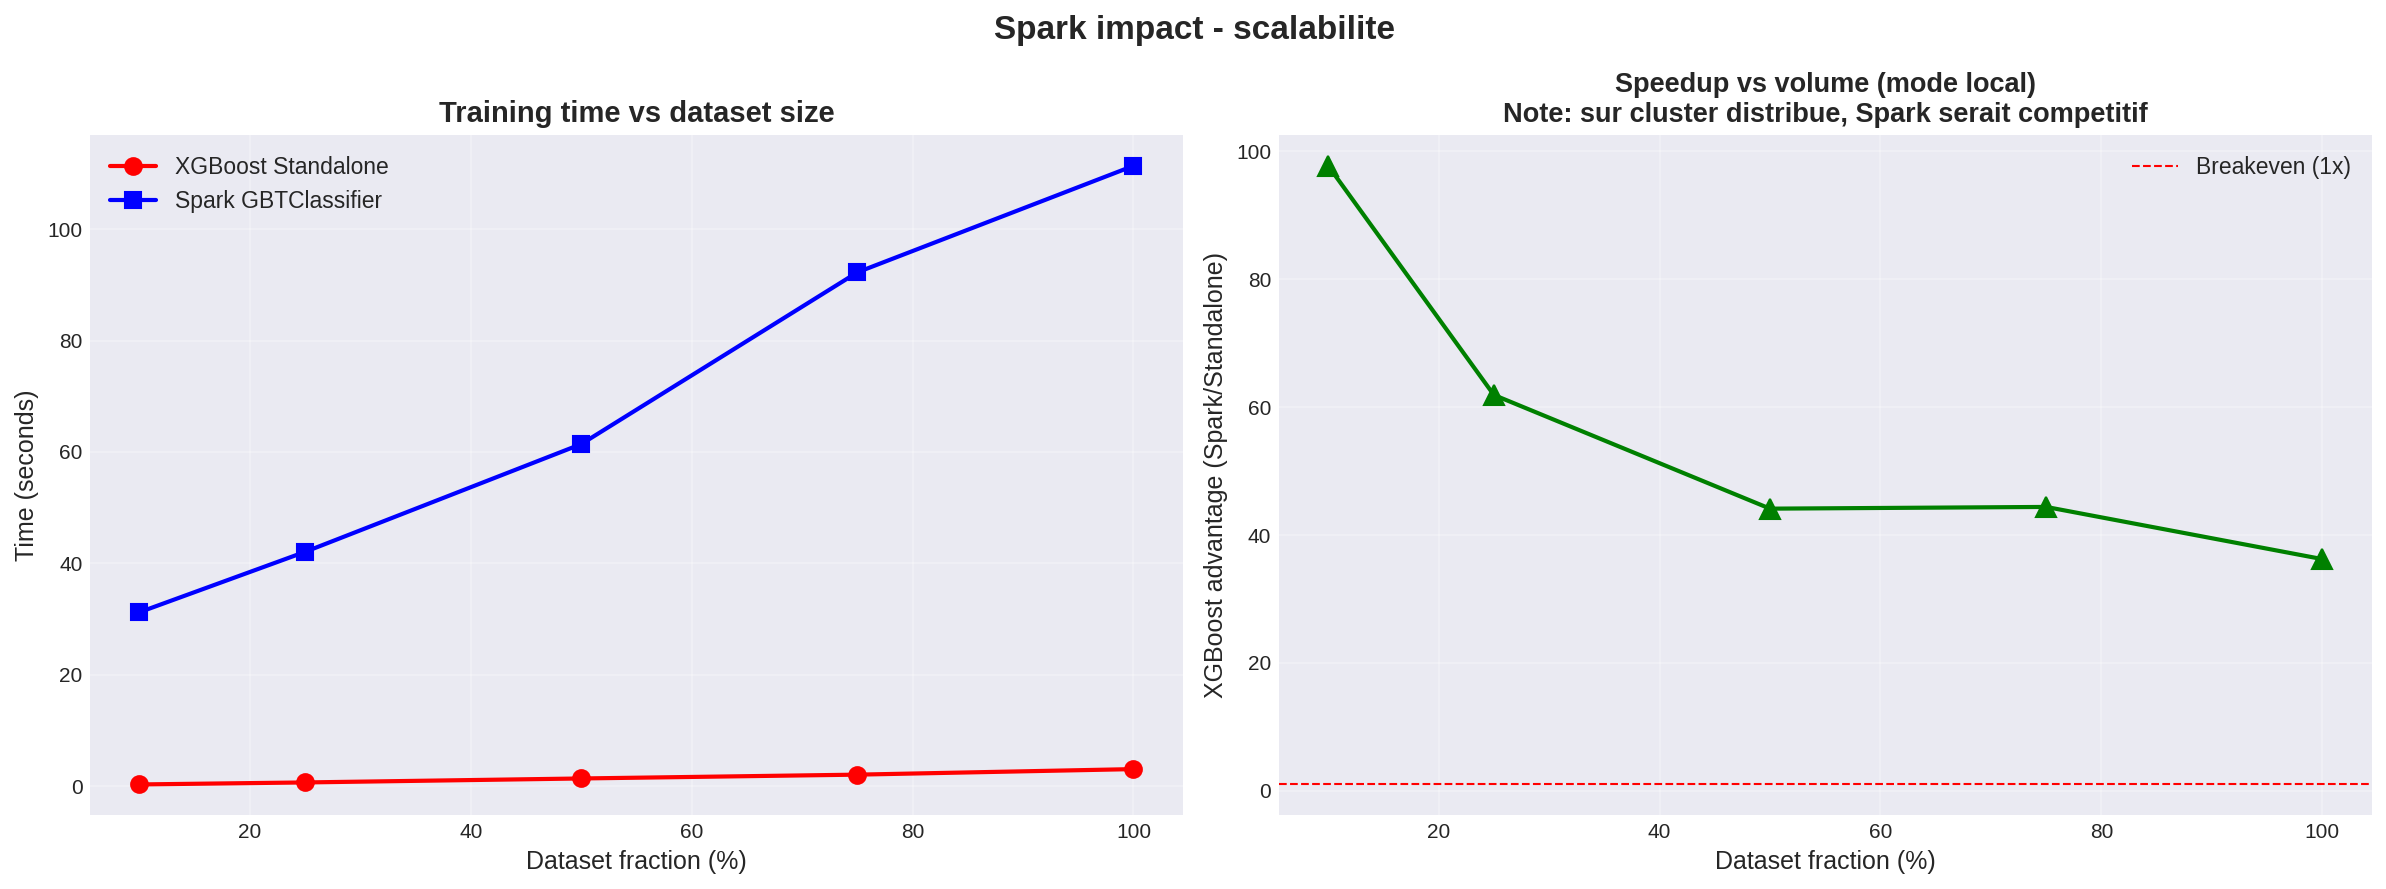
\includegraphics[width=\textwidth]{figures/spark_scalability.png}
    \caption{Comparaison des temps d'entraînement Spark GBT et XGBoost standalone
             en fonction de la taille du jeu de données (gauche), et facteur
             d'avantage XGBoost correspondant (droite). En mode local sur
             une seule machine, XGBoost est 36 à 98 fois plus rapide que Spark GBT.}
    \label{fig:scalability}
\end{figure}

L'écart observé (36 à 97 fois) traduit l'overhead inhérent à Spark en mode local~:
sérialisation des données, communication entre le pilote et les exécuteurs,
et démarrage de la JVM. Sur un cluster distribué de huit nœuds ou plus,
Spark deviendrait compétitif pour des volumes dépassant 10~millions de lignes,
conformément aux résultats publiés par Zhang et al.~\cite{zhang2023}.

% ─────────────────────────────────────────────────────────────────────────────
\section{Phase 6 : Tableau de bord Streamlit}
% ─────────────────────────────────────────────────────────────────────────────

Le tableau de bord Streamlit est une application multi-pages découplée du pipeline
d'entraînement. Elle charge des artefacts pré-calculés (fichiers JSON, CSV et PNG)
depuis un dossier \texttt{results/} et peut être exécutée localement sans Spark ni
modèle chargé en mémoire. L'application est structurée en une page d'accueil et
trois pages d'analyse thématiques.

\subsection{Page d'accueil}

La page d'accueil (figure~\ref{fig:streamlit_home}) présente les quatre indicateurs
clés du projet~: nombre total d'observations, nombre de variables, prévalence MCV
et meilleur AUC-ROC obtenu. Elle donne également un aperçu de la stack technique et
oriente l'utilisateur vers les trois pages d'analyse via le menu latéral.

\begin{figure}[H]
    \centering
    \includegraphics[width=\textwidth]{figures/streamlit_accueil.png}
    \caption{Page d'accueil du tableau de bord Streamlit --- indicateurs clés du
             projet (observations, variables, prévalence MCV, AUC-ROC) et
             description de la stack technique.}
    \label{fig:streamlit_home}
\end{figure}

\subsection{Page EDA — Exploration des données}

La page EDA (figure~\ref{fig:streamlit_eda}) permet d'explorer interactivement
le dataset BRFSS sur un échantillon de 100\,000 lignes. Elle propose~:
\begin{itemize}
    \item des filtres latéraux par sexe et tranche d'âge appliqués dynamiquement ;
    \item la distribution de la variable cible (camembert et histogramme) ;
    \item les distributions univariées de chaque feature par classe (MCV / non-MCV) ;
    \item les matrices de corrélation de Pearson et Spearman et l'évolution du taux
          de MCV par tranche d'âge.
\end{itemize}

\begin{figure}[H]
    \centering
    \includegraphics[width=\textwidth]{figures/streamlit_eda.png}
    \caption{Page EDA du tableau de bord --- exploration interactive des distributions
             du dataset BRFSS 2020--2024 avec filtres par sexe et tranche d'âge.}
    \label{fig:streamlit_eda}
\end{figure}

\subsection{Page Résultats des modèles}

La page Résultats (figure~\ref{fig:streamlit_models}) compare les performances
du DNN et d'XGBoost via~:
\begin{itemize}
    \item un sélecteur de seuil DNN (optimal F1 ou défaut 0,5) dans la barre latérale ;
    \item cinq indicateurs KPI (accuracy, précision, rappel, F1-score, AUC-ROC) ;
    \item les courbes ROC superposées, les matrices de confusion et le graphique
          d'impact du seuil sur les métriques ;
    \item les importances de features XGBoost (critères weight, gain et cover).
\end{itemize}

\begin{figure}[H]
    \centering
    \includegraphics[width=\textwidth]{figures/streamlit_models.png}
    \caption{Page Résultats des modèles --- comparaison DNN vs XGBoost avec
             sélecteur de seuil interactif, courbes ROC et matrices de confusion.}
    \label{fig:streamlit_models}
\end{figure}

\subsection{Page Impact Spark}

La page Impact Spark (figure~\ref{fig:streamlit_spark}) présente~:
\begin{itemize}
    \item les temps d'entraînement des trois modèles (DNN, XGBoost, Spark GBT)
          sous forme de KPI et d'histogramme~;
    \item le graphique de scalabilité Spark vs XGBoost standalone sur cinq fractions
          croissantes du dataset~;
    \item le facteur d'avantage XGBoost (36 à 97 fois) en fonction du volume~;
    \item une synthèse de la valeur ajoutée de Spark dans chaque phase du pipeline.
\end{itemize}

\begin{figure}[H]
    \centering
    \includegraphics[width=\textwidth]{figures/streamlit_spark.png}
    \caption{Page Impact Spark --- benchmark XGBoost standalone vs Spark GBTClassifier
             sur cinq fractions du jeu de données (10\% à 100\%), avec facteur
             d'avantage et analyse de la valeur ajoutée du traitement distribué.}
    \label{fig:streamlit_spark}
\end{figure}

Les chemins de fichiers sont résolus de façon portable via \texttt{Path(\_\_file\_\_).parent},
et les fonctions de chargement gèrent les fichiers manquants par un avertissement
non bloquant, garantissant la robustesse de l'application en cas de résultats
partiels. L'application est lancée par la commande \texttt{streamlit run app.py}
depuis le dossier \texttt{streamlit\_dashboard/}.
